%\part*{Lezione 01/03/2021}
\chapter{Modelli nucleari}
In questo capitolo introduciamo e discutiamo i modelli nucleari \textit{a shell} e \textit{a goccia}. Il capitolo copre le Lezioni del 01/03/2021 e del 03/03/2021.

\paragraph{Introduzione} Se il sistema a due nucleoni è \vir{complicato}, quando $A$ diviene proibitivo è necessario ricorrere a modelli per descrivere le proprietà nucleari\footnote{Per un testo di riferimento sull'argomento vedi \complrif{compl-krane}.}. Dall'analogia con la fisica atomica, il modello \vir{più semplice} che approfondiremo per primo è appunto un modello di tipo \textit{a shell}.

\section{Primi passi per il modello \textit{a shell}}
Nel caso della fisica atomica un modello \textit{a shell} è supportato dagli andamenti del raggio atomico e dell'energia di ionizzazione (Figura \ref{0301_rE}), i cui salti possono essere associati  appunto alla \vir{chiusura} di uno \textit{shell}. In questo modello gli elettroni si muovono in un campo esterno generato dal nucleo, senza collidere tra loro.\\
Applicare tutto ciò alla fisica nucleare non è immediato: i nucleoni, infatti, \vir{vivono} in un potenziale che non è esterno, ma generato da essi stessi e le loro dimensioni non sono trascurabili rispetto alle dimensioni del nucleo.
\begin{figure}[!h]
    \centering
    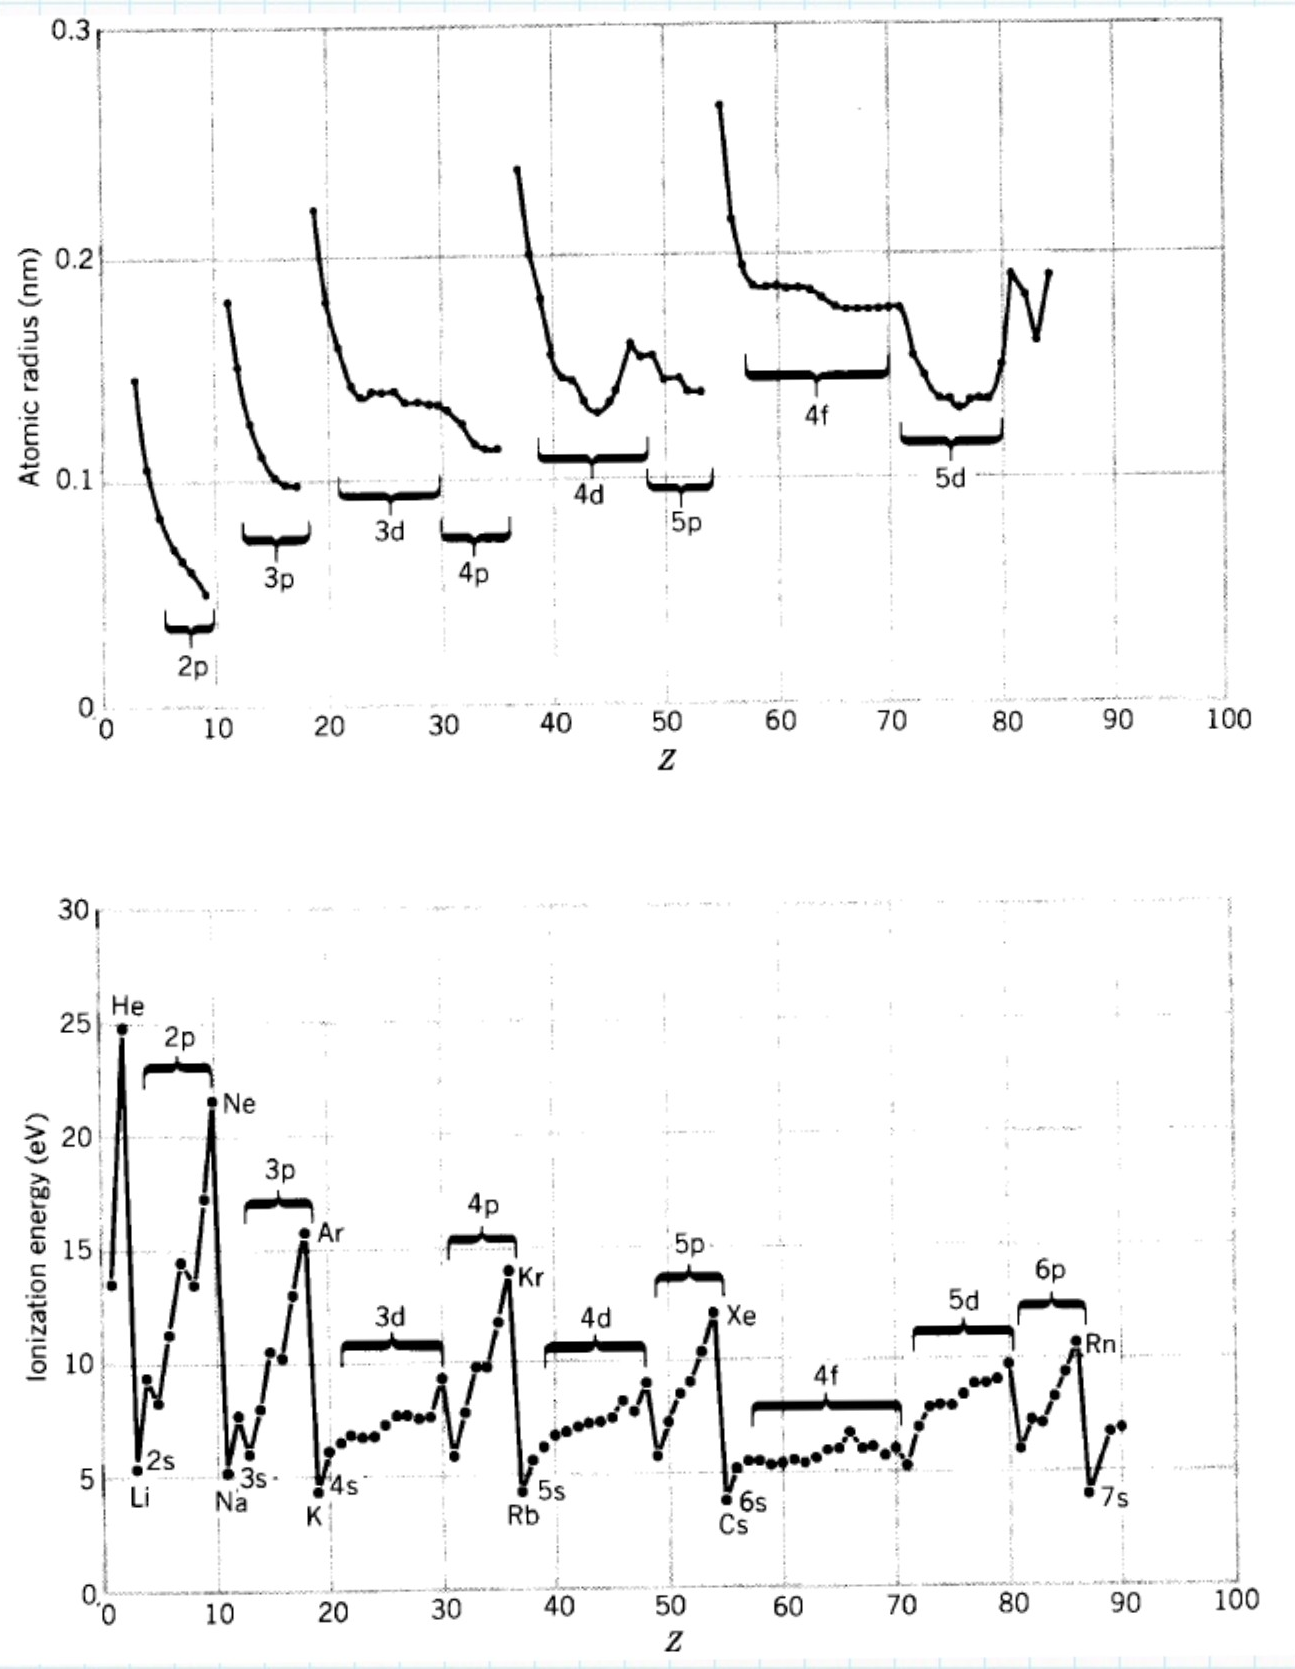
\includegraphics[scale=0.2]{Immagini/ratm-Eion.png}
    \caption{Andamento in alto del raggio atomico e in basso dell'energia di ionizzazione al variare del numero atomico. I salti sono ben spiegati da un modello \textit{a shell}.}
    \label{0301_rE}
\end{figure}
\newline
Tuttavia, vi sono alcune evidenze sperimentali a favore di tale modello. Innanzitutto, le differenze di energia di separazione\footnote{Sono le energie di separazione del protone e del neutrone rispettivamente.} tra nuclei con $N=\mbox{cost}$ (\textbf{isotoni}\index{nucleo!isotono}) e nuclei con $Z=\mbox{cost}$ (\textbf{isotopi}\index{nucleo!isotopo}) hanno salti ben determinati\footnote{Dovrebbe comparire anche il 2, ma non lo vedo perché corrisponde alla separazione di 2 protoni. Per quanto riguarda il 126 non si vede in natura nel caso di $Z$, perché il nucleo non è stabile.}, come mostrato in Figura \ref{diffeng}. I numeri atomico o neutronico per i quali si hanno i salti richiamano i numeri quantici di un modello \vir{a shell} e vengono definiti \textbf{numeri magici}\index{numeri magici}:
$$2,8,20,28,50,82,126$$
\begin{figure}[!h]
    \centering
    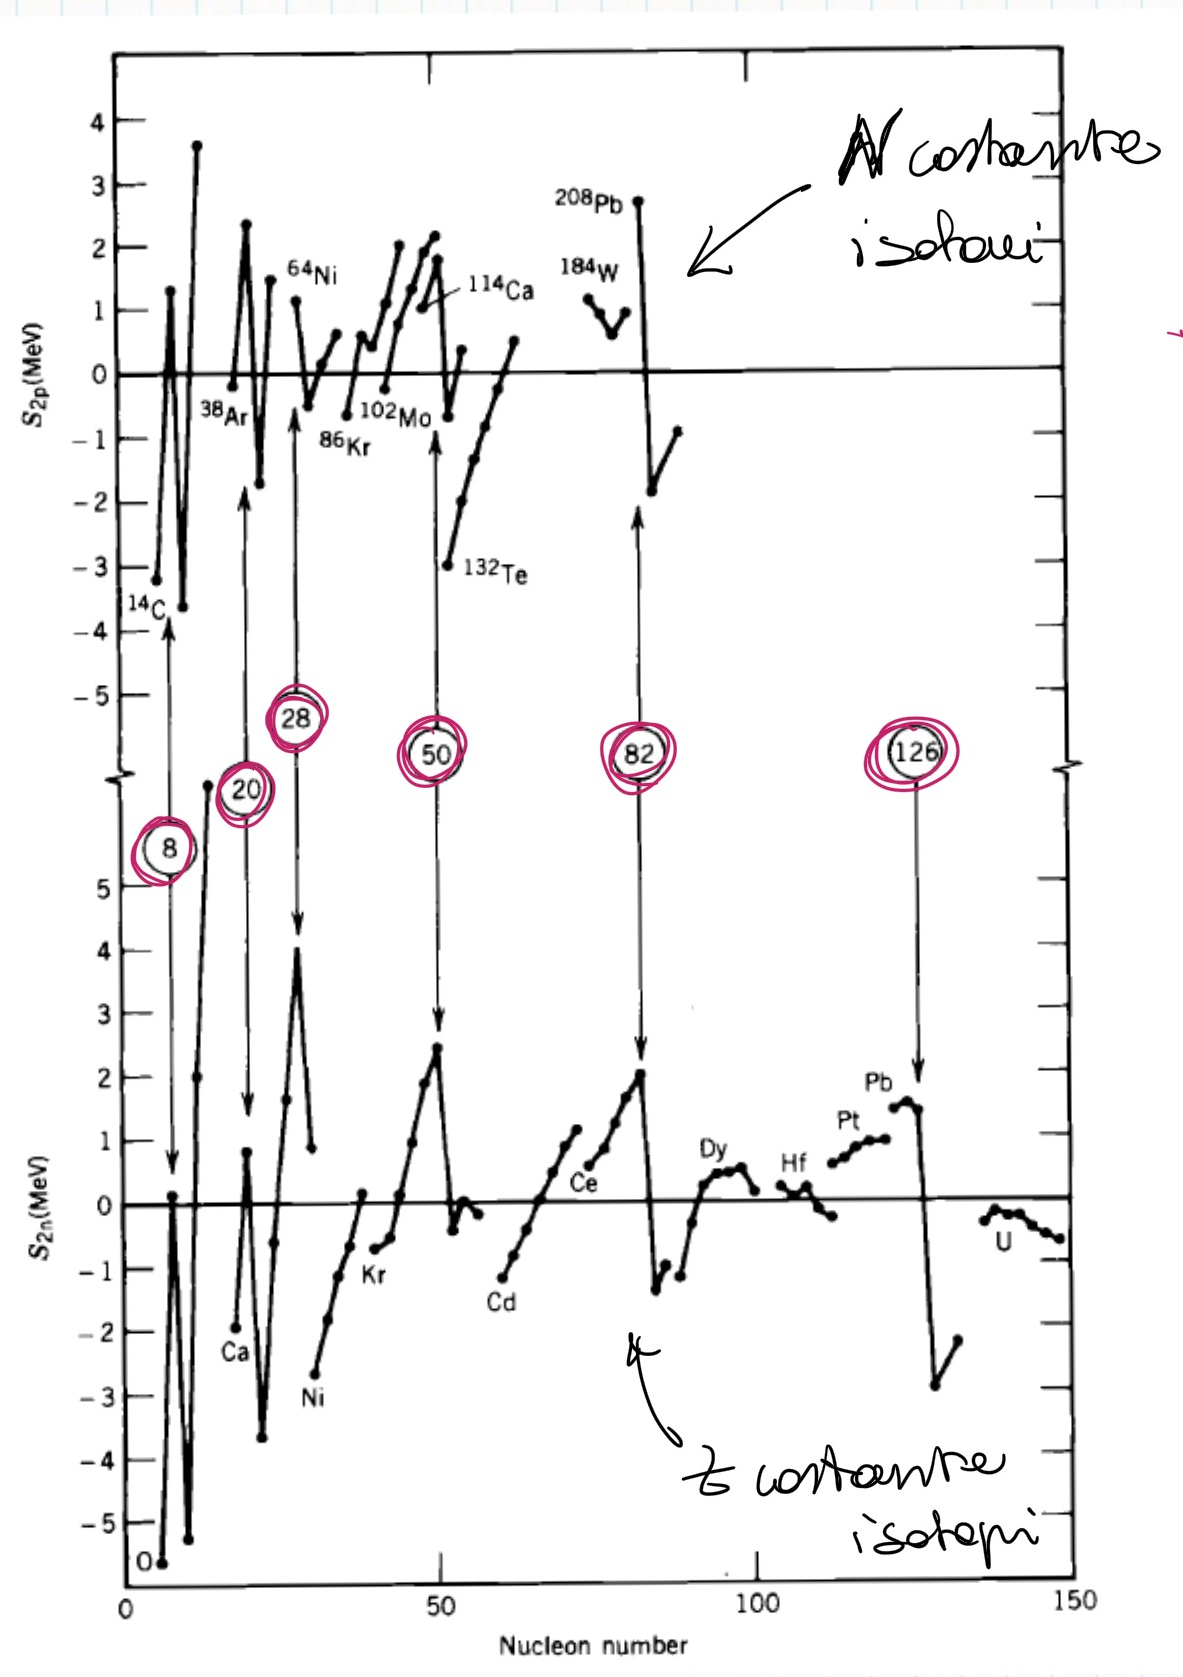
\includegraphics[scale=0.2]{Immagini/mag-num.png}
    \caption{In alto l'andamento dell'energia di separazione degli isotoni $S_n$ e in basso quello dell'energia di separazione degli isotopi $S_p$. Al centro sono riportati i numeri magici.}
    \label{diffeng}
\end{figure}

\noindent Un'altra evidenza consiste negli andamenti della sezione d'urto di cattura neutronica $\sigma$ e dei raggi di carica nucleari, riportati in Figura \ref{sigmar}, che ricordano quello del raggio atomico.

\begin{figure}[!h]
    \centering
    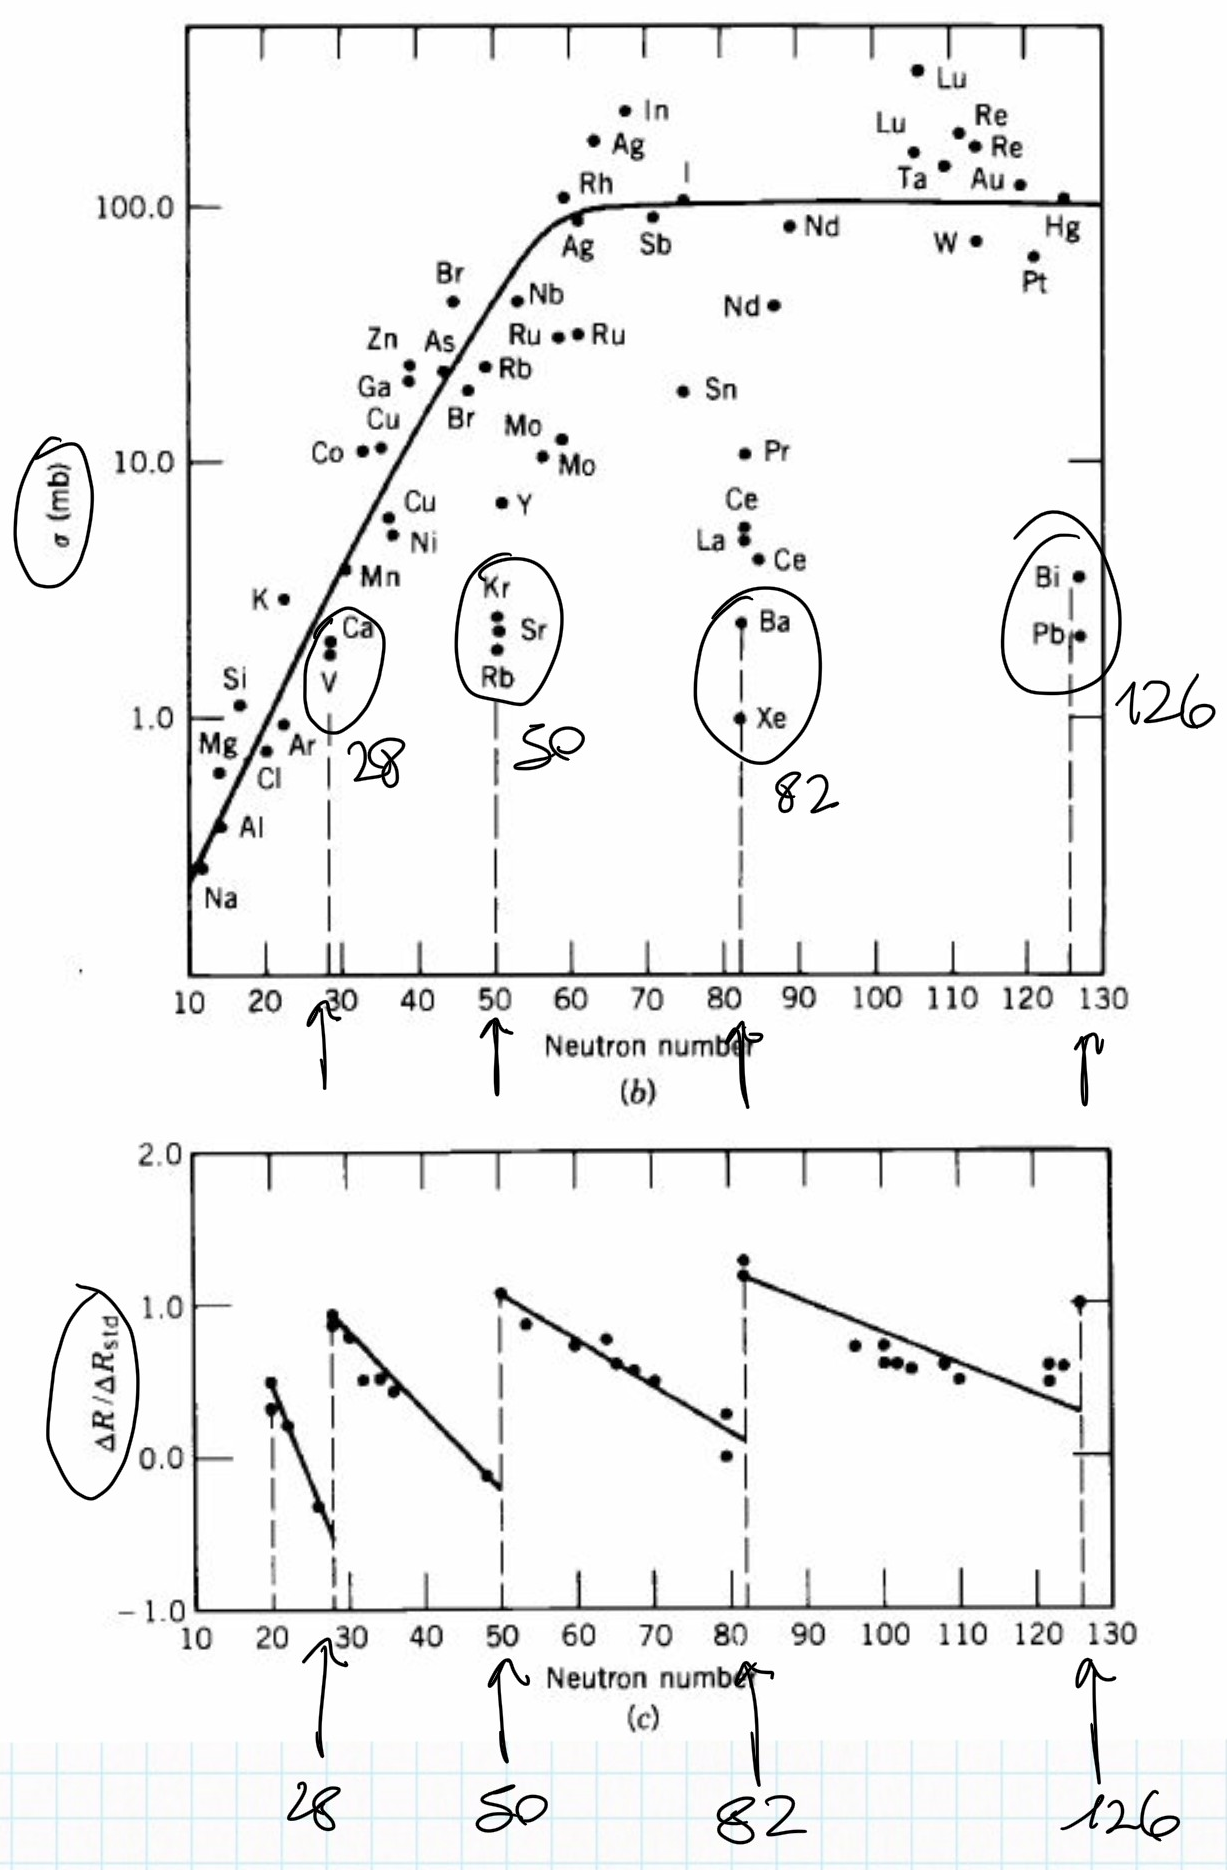
\includegraphics[scale=0.3]{Immagini/mag-num2.png}
    \caption{Andamenti della sezione d'urto $\sigma$ in alto e dei raggi di carica in basso in funzione del numero di neutroni nel nucleo. Si osservano salti in corrispondenza dei numeri magici.}
    \label{sigmar}
\end{figure}
\newpage
\section{Modello \textit{a shell}}
\index{modelli nucleari! a shell@\textit{a shell}}
\subsection{Sciogliamo i nodi} 
Innanzitutto risolviamo i problemi che ci eravamo posti nella formulazione del modello.
Assumiamo che il moto del singolo nucleone sia governato dal potenziale generato da tutti gli altri con i quali interagisce, escluso esso stesso. Per quanto riguarda gli urti, essendo i nucleoni fermioni se avvenisse una collisione (quindi un trasferimento di energia) questo comporterebbe una promozione a un livello di valenza (unico disponibile per Pauli), ma le energie richieste per far ciò sono notevolmente maggiori di quelle scambiabili attraverso l'urto. Dunque, assumeremo che gli urti non avvengono.\\[-1cm]
\paragraph{Calcolo della funzione d'onda} Dobbiamo ovviamente soddisfare all'equazione di \Sch, tuttavia per semplificare il calcolo possiamo prima rimaneggiare l'hamiltoniana del sistema: 
$$H=\sum_i T_i + \sum_{i<j}V_{ij}$$ 
con $T_i$ l'energia cinetica e $V_{ij}$ il potenziale di interazione. Sommando e sottraendo il potenziale $U_i$ che sente la $i$-esima particella a causa degli altri $j\not =i$ nucleoni, si ottiene:
\begin{displaymath}
\begin{aligned}
H&=\sum_i T_i + \sum_{i<j}V_{ij} +\sum_i U_i - \sum_i U_i=\\
&= \sum_i (T_i + U_i) + \Bigl [ \sum_{i<j} V_{ij} - \sum_i U_i \Bigr ] \simeq\\
&\simeq \sum_i (T_i + U_i)\\
H_i &\simeq T_i + U_i
\end{aligned}
\end{displaymath}
dove nell'ultimo passaggio abbiamo trascurato il contributo dato dal potenziale residuo, perché se $U_i$ è una buona approssimazione del campo che risente $i$ allora quella differenza è molto \vir{piccola}. Otteniamo così un'hamiltoniana di singola particella, per cui $H_i \psi_i = \varepsilon_i \psi_i$, con $\psi = \Pi_i \psi_i$ e $E = \sum_i \varepsilon_i$. Data la natura dei fermioni, cerchiamo una $\psi$ antisimmetrica, che otteniamo tramite il determinante di Slater\footnote{Per puro scopo esemplificativo riportiamo il caso $N=2$:
$$\psi (\xi_1,\xi_2) = \psi_1 (\xi_1)\psi_2 (\xi_2) - \psi_2 (\xi_1)\psi_1 (\xi_2)$$}:
\begin{displaymath}
\psi = \det
\begin{vmatrix}
\psi_1 (\xi_1) & \psi_1 (\xi_2) & \dots & \psi_1 (\xi_N) \\
\psi_2 (\xi_1) & \psi_2 (\xi_2) & \dots & \psi_2 (\xi_N) \\
\vdots         &                & \ddots&                \\
\psi_N (\xi_1) & \psi_N (\xi_2) & \dots & \psi_N (\xi_N)
\end{vmatrix}
\end{displaymath}
Rimane quindi da scegliere il potenziale $U_i$.
\begin{itemize}
    \item \textbf{Potenziale a buca infinita}: conosciamo già la soluzione per gli stati legati\footnote{Mettiamo $\hbar=1$.}, ovvero $\psi = A \sin (kx) + B \cos (kx)$, con $k\equiv \sqrt{2mE}$. Dalle condizioni ai bordi $\psi(0)=\psi(a)=0$, si ha $ka = n\pi$ per cui $\varepsilon_n = \hbar^2 \pi^2  n^2 / 2ma^2$.
    \item \textbf{Potenziale armonico} $V(x)=Kx^2/2$: anche in questo caso sappiamo che le soluzioni sono della forma $\psi(x) = H(x)\exp{(-\alpha x^2/2)}$, con $\alpha \equiv \sqrt{Km}$ e $H(x)$ polinomio di Hermite, il cui grado dà l'energia. Si ha quindi nel caso unidimensionale $\varepsilon_n = \hbar \omega_0 (n+1/2)$, dove $\omega_0 \equiv \sqrt{K/m}$, da cui generalizzando $E_N= \hbar \omega_0 (N+3/2)$, con $N= n_x+n_y+n_z$.
    \item \textbf{Buca Wood-Saxon}\index{buca di Wood-Saxon}: in questo caso il conto è un po' più complicato, lo vedremo successivamente; intanto riportiamo soltanto l'espressione di questo potenziale:
    $$V(x) = - \frac{V_0}{1+\exp{(\frac{r-R}{a})}}$$
    dove $V_0$ è la profondità della buca in $r=0$, $R$ è il raggio medio e $a$ è quella che viene chiamata \textit{skin thickness}\footnote{Questi dettagli sono stati presi da Krane, K., S., \textit{\vir{Introductory Nuclear Physics}}, USA, John Wiley \& Sons, 1988.}.
\end{itemize}
\noindent Come per il modello \textit{a shell} atomico usiamo la notazione spettroscopica per cui $N = 2(n-1)+\ell$, dove $n$ non è però il numero quantico principale (tiene conto solo del numero di livelli con un certo $\ell$) e $\ell$ è il momento angolare. Considerando anche lo \textit{spin}, abbiamo una \textbf{degenerazione dello stato energetico} pari a: $2(2\ell+1)$, per cui:
\begin{displaymath}
\begin{aligned}
&N & n&,\ell & \text{orb}&\text{itale} & \text{Numero}&\text{ nucleoni} & \text{To}&\text{tale}\\
&0 & 1&,0 & &1s & &2 & &2   \\
&1 & 1&,1 & &1p & &6 & &8   \\
&2 & 1,2&;2,0 & 1d&;2s & 10&+2 & &20 \\
&3 & 1,3&;2,1 & 1f&;2p & 14&+6 & &40   \\
&4 & 1,4;2&,2;3,0 & 1g;2&d;3s & 18+&10+2 & &70
\end{aligned}
\end{displaymath}
Osserviamo che il numero totale di nucleoni nei primi 3 livelli pieni corrisponde proprio ai primi 3 numeri magici, ma dal quarto in poi la sequenza non è più rispettata; con questo tipo di potenziale infatti riesco a spiegare bene solo le prime 3 configurazioni, come mostrato in Figura \ref{shell} e in Figura \ref{shellmix} a sinistra.
\begin{figure}[h]
    \centering
    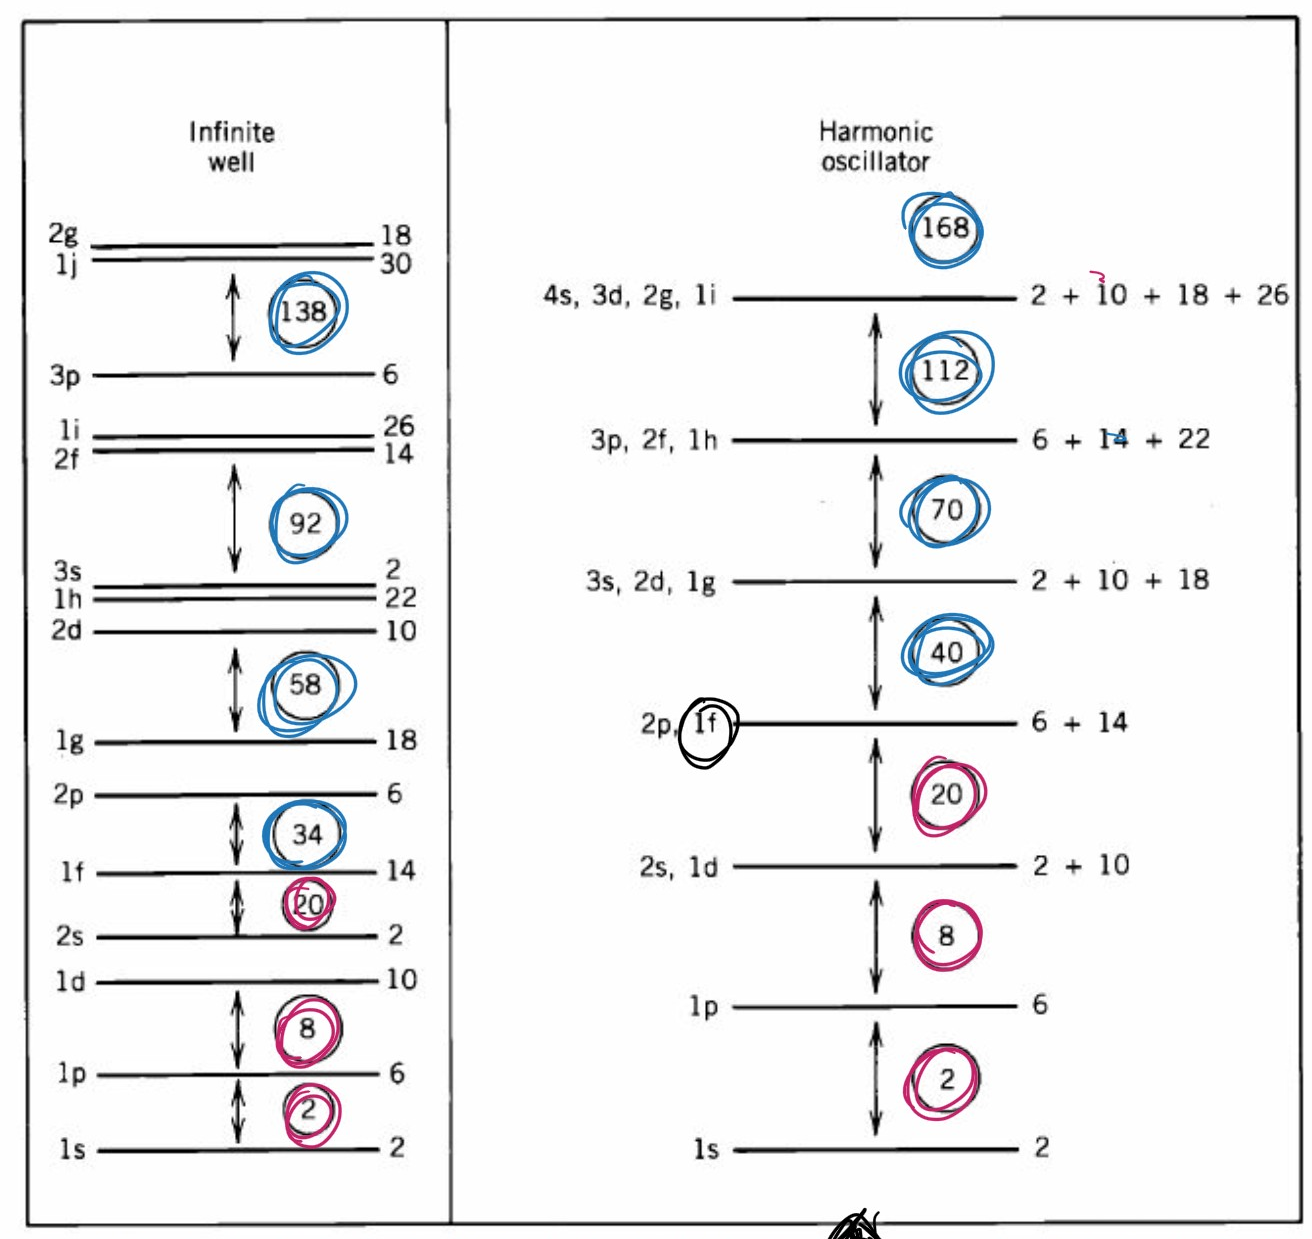
\includegraphics[scale=0.25]{Immagini/shell.png}
    \caption{Sequenza degli orbitali a sinistra con potenziale a buca e a destra con potenziale armonico.}
    \label{shell}
\end{figure}

\subsection{Modello \textit{a shell} + spin-orbita}
Consideriamo adesso il potenziale di Wood-Saxon (più realistico della buca e dell'armonico) e teniamo conto dell'interazione \textit{spin}-orbita\footnote{Di questa ne abbiamo evidenze nello scattering neutrone-neutrone}:
$$U (r) = V_{WS}(r) +  V_{s-o}(r)\; \vec{\ell} \cdot \vec{s} $$
$$ H \to T+V_{WS}(r)+V_{s-o}(r)\;\vec{\ell} \cdot \vec{s}$$
dove abbiamo omesso le $i$ ai pedici per semplicità. Aver introdotto questa interazione, però, rende $\ell_z$ e $s_z$ non più dei buoni numeri quantici poiché non commutano con $\vec{\ell}\cdot\vec{s}$; consideriamo allora il momento angolare totale $\vec{j}= \vec{\ell} + \vec{s}$ ed esprimiamo $\vec{\ell}\cdot\vec{s}$ in funzione di $j$ (per il singolo nucleone):
$$\mean{\vec{\ell}\cdot\vec{s}} = \frac{1}{2}\Bigl[j(j+1) - \ell(\ell+1) - \frac{3}{4} \Bigr]$$
Proviamo a questo punto a descrivere la configurazione $1f$ ($n=1,\ell=3$), che era la prima a non rispettare la sequenza dei numeri magici: abbiamo $j=5/2,7/2$ con degenerazione $2j+1$, per cui $1f_{5/2}$ ha 6 nucleoni e $1f_{7/2}$ ha 8 nucleoni\footnote{Questo ci piace perché sommato all'orbitale precedente si ottiene proprio 28.}. Per fare i conti, supponiamo che $V_{s-o}$ sia una buca rettangolare di profondità $V_0$, allora:
$$\diag{1f_{7/2}}{U_{s-o}} \sim - \frac{V_0}{2}\Bigl[ \frac{7}{2}\cdot\frac{9}{2} - 3\cdot 4 - \frac{3}{4} \Bigr] = -\frac{3}{2} V_0$$
$$\diag{1f_{5/2}}{U_{s-o}} \sim - \frac{V_0}{2}\Bigl[ \frac{5}{2}\cdot\frac{7}{2} - 3\cdot 4 - \frac{3}{4} \Bigr] = 2 V_0$$
Abbiamo che i due stati sono separati e la configurazione $1f_{7/2}$ si avvicina agli orbitali precedenti, per cui si ha un rimescolamento degli \textit{shell} che determina la sequenza dei numeri magici, come mostrato in Figura \ref{shellmix}.
\begin{figure}[h]
    \centering
    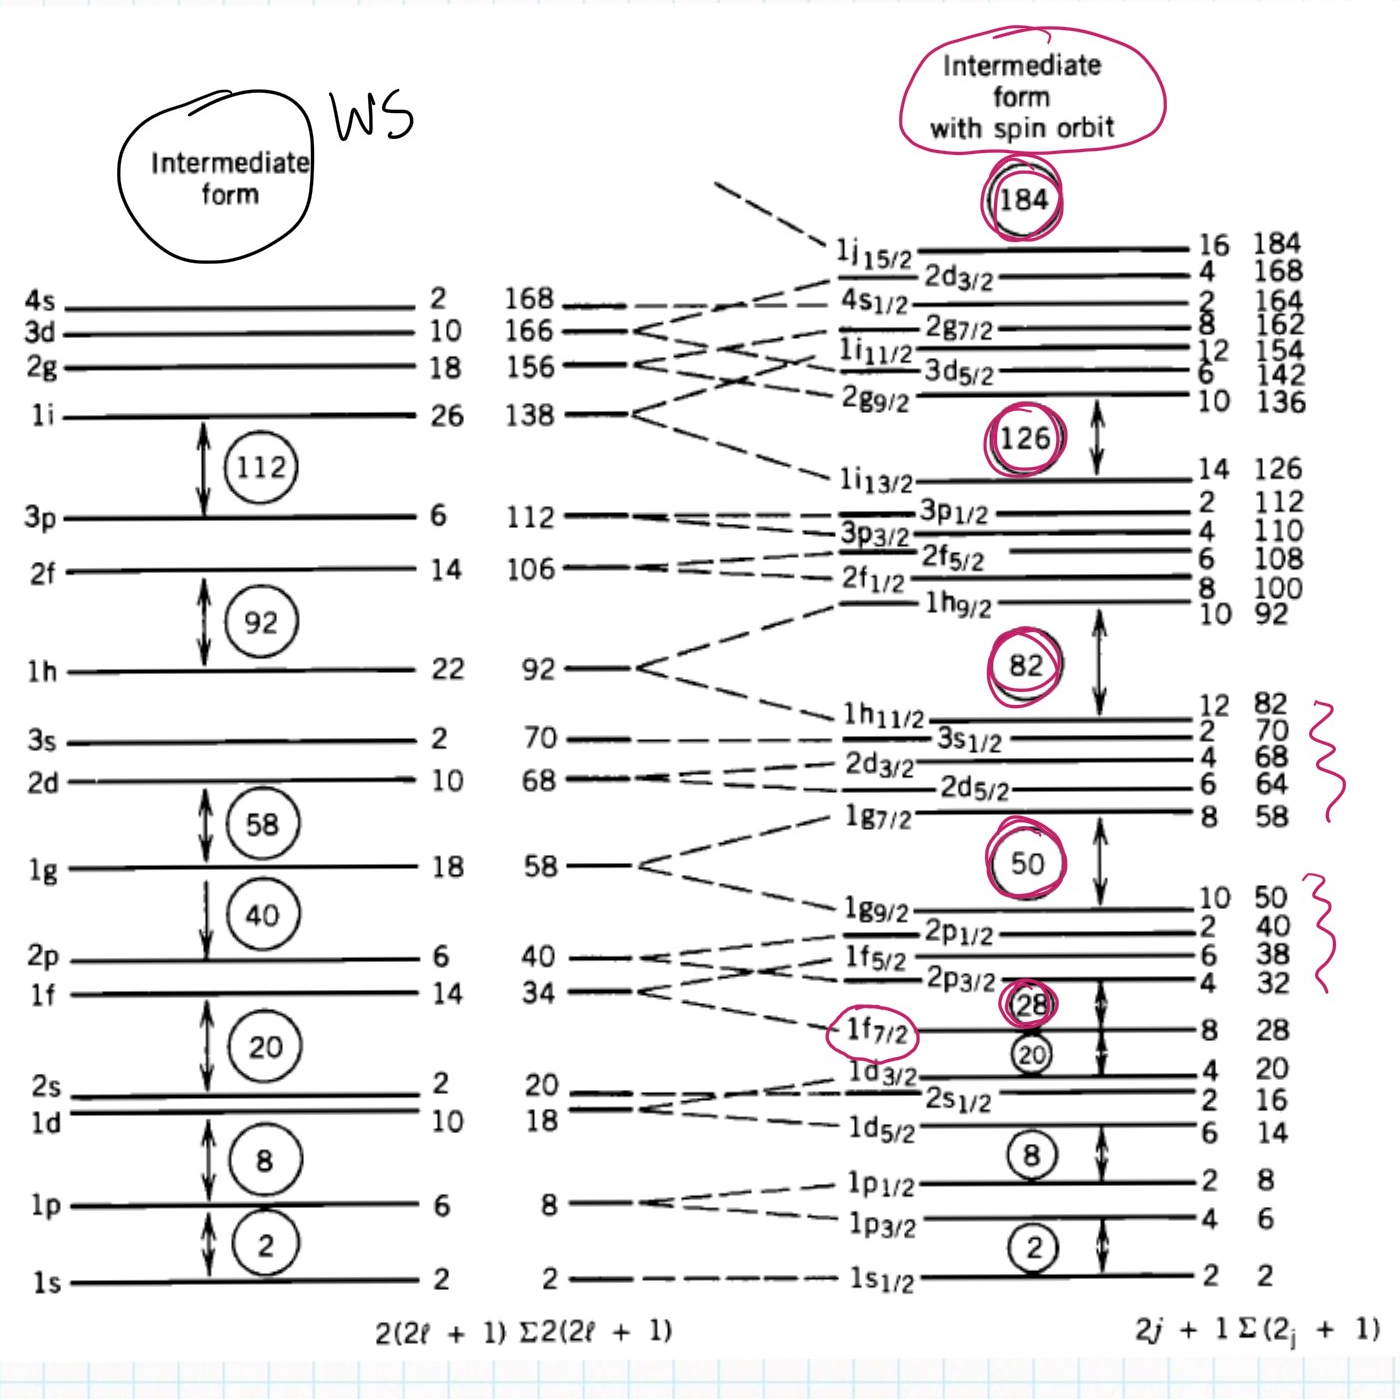
\includegraphics[scale=0.3]{Immagini/shell2.png}
    \caption{Configurazioni degli orbitali a sinistra con un potenziale di Wood-Saxon senza interazione \textit{spin}-orbita e a destra con lo stesso potenziale ma considerando tale interazione. Si vedono i rimescolamenti degli \textit{shell} e i numeri magici. Nella figura è presente un errore: è segnato $2f_{1/2}$ invece di $2f_{7/2}$.}
    \label{shellmix}
\end{figure}
%\noindent Dalla figura vediamo che c'è uno \textit{splitting} anche nella configurazione $1p$ e in altre, ma questi sono piccolissimi.

\subsubsection{I successi del modello} 
Questo modello è valso un premio Nobel, non solo perché riproduce i numeri magici, ma anche perché spiega varie evidenze sperimentali. Per esempio, giustifica il fatto che nuclei doppiamente magici, ovvero con sia $N$ che $Z$ numeri magici (come $\ce{^4_2He_2}$, $\ce{^{16}_8O_8}$,\dots), siano fortemente legati e la presenza del $J^\pi = 0^+$ per il fondamentale di tutti i nuclei pari-pari (tutti i nucleoni sono accoppiati). Il modello\footnote{In realtà questo è \textit{extreme indipendent particle model}.}, infatti, permette di descrivere le prorpietà dell'intero sistema dallo stato di un singolo nucleone spaiato.
Maggior successo fu appunto la previsione del $J^\pi$ dei nuclei pari-dispari. Prendiamo a esempio $\ce{^{17}_8O_9}$: osserviamo che, secondo il modello, ha un neutrone spaiato nel livello $1d_{5/2}$ ed è di conseguenza questo che determina il $J^\pi$ del nucleo nel fondamentale, che è appunto $J^\pi=\frac{5}{2}^+$. Il $\ce{^15_8O_7}$ ha invece un neutrone spaiato nello stato $1p_{1/2}$, quindi $J^\pi = \frac{1}{2}^-$. In realtà, questo modello funziona solo per i nuclei con $A$ dispari e $A<150 \vee 190<A<220$, ma è un aspetto che approfondiremo più avanti.\\
Altro successo del modello è la predizione dei momenti di dipolo magnetico nucleare $\vec{\mu} = \mu_N (g_\ell \vec{\ell}+g_s \vec{s})$, dove $g_\ell$ è il fattore giromagnetico per il momento angolare orbitale e $g_s$ per lo \textit{spin}\footnote{Ricordiamo che nel caso del protone $g_\ell = 1$ e $g_s=g_s^p = 5.58$, mentre nel caso del neutrone $g_\ell = 0$ e $g_s=g_s^n = -3.82$.}:
$$\mu \equiv \mean{\frac{\vec{\mu}\cdot\vec{j}\, j_z}{j^2}} = \frac{j}{j(j+1)}\mean{\vec{\mu}\cdot\vec{j}}$$
Calcoliamoci allora $\mean{\vec{\mu}\cdot\vec{j}}$, sfruttando $(\vec{j}-\vec{\ell})^2 = j^2 + \ell^2 -2\vec{j}\cdot\vec{\ell}$ e $(\vec{j}-\vec{s})^2 = j^2 + s^2 - 2\vec{j}\cdot\vec{s}$:
\begin{displaymath}
\begin{aligned}
\mean{\vec{\mu}\cdot\vec{j}} &= \mu_N \Bigl (g_\ell \mean{\vec{\ell}\cdot\vec{j}} +g_s \mean{\vec{s}\cdot\vec{j}} \Bigr ) = \\
&= \frac{\mu_N}{2} \Bigl [g_\ell (j^2 + \ell^2 - s^2) + g_s (j^2-\ell^2+s^2) \Bigr ] \\
\mu &= \frac{\mu_N}{2(j+1)} \Bigl [(g_\ell+g_s) j(j+1) + (g_\ell-g_s) (\ell(\ell+1)-s(s+1)) \Bigr ]
\end{aligned}
\end{displaymath}
Poiché $s=1/2$, si ha $\ell=j\pm 1/2$, per cui:
$$\mu = \Bigl \{
\begin{array}{ll}
    \mu_N [g_\ell (j-1/2)+g_s/2] & j = \ell+1/2 \\
    \mu_N [g_\ell \frac{j(j+3/2)}{j+1}- g_s \frac{j}{2(j+1)}] & j = \ell -1/2 
\end{array}$$
Vediamo alcuni risultati sperimentali per il neutrone e per il protone in Figura \ref{curve}, dove sono riportate le \textbf{linee di Smith}\index{linee di Smith} per i vari andamenti (ovvero il conto teorico). Si osserva che il modello riproduce solo qualitativamente i dati, che sembrano \textit{shiftati} di una certa quantità e ciò è dovuto al fatto che le linee sono ottenute usando i valori di $g_\ell$ e $g_s$ del nucleone libero, invece di tenere in conto che il nucleone è \vir{immerso} in un mezzo denso; questa correzione viene chiamata \textit{medium modification}.\\
Per quanto riguarda il momento di quadrupolo elettrico il modello riesce a dare una predizione dell'andamento.
$$Q_{ij} = \sum_\text{part. cariche} 3x_ix_j -r^2\delta_{ij}$$
Quello che viene misurato è $Q_{zz} = 3z^2 - r^2$, che va calcolato sugli stati con $p$ spaiato\footnote{Ovviamente se calcolato per $n$ spaiato troviamo $\mean{Q} = 0$ esattamente.}. Si trova così:
$$\mean{Q} = -\frac{2j-1}{2(j+1)}\mean{r^2}\qquad \text{con } \mean{r^2} = \frac{3}{5}R^2 =\frac{3}{5}R_0^2A^{2/3}$$
che va valutato per $j=\ell\pm 1/2$. Riportiamo in Figura \ref{Q} gli andamenti dei dati sperimentali, dove si osserva che per $Z$ o $N$ \vir{grandi} si perde l'accordo con la teoria.

\subsubsection{I problemi del modello} 
Partiamo proprio dall'ultimo grafico, quello in Figura \ref{Q}. Notiamo che per circa $Z>50$ non vi è accordo, ma soprattutto per circa $N>100$ compaiono momenti di quadrupolo elettrico per i neutroni e questo è assurdo! Si potrebbe cercare di spiegare questa evidenza imputando la presenza di questi quadrupoli ai protoni degli \textit{shell} precedenti più vicini, ma in realtà non è così\footnote{Le linee nella figura sono proprio ottenute con queste correzioni e come si vede non rappresentano i dati}. Per questi nuclei, dunque, il modello \textit{a shell} non è sufficiente a spiegare tali evidenze, poiché non tiene conto di alcun tipo di moti collettivi, ma imputa la totale descrizione del sistema al solo nucleone spaiato\footnote{Tuttavia, in questo caso anche considerare più nucleoni spaiati non fornisce osservabili compatibili.}. Vedremo che è necessario introdurre un nuovo modello.

\begin{figure}[!h]
    \centering
    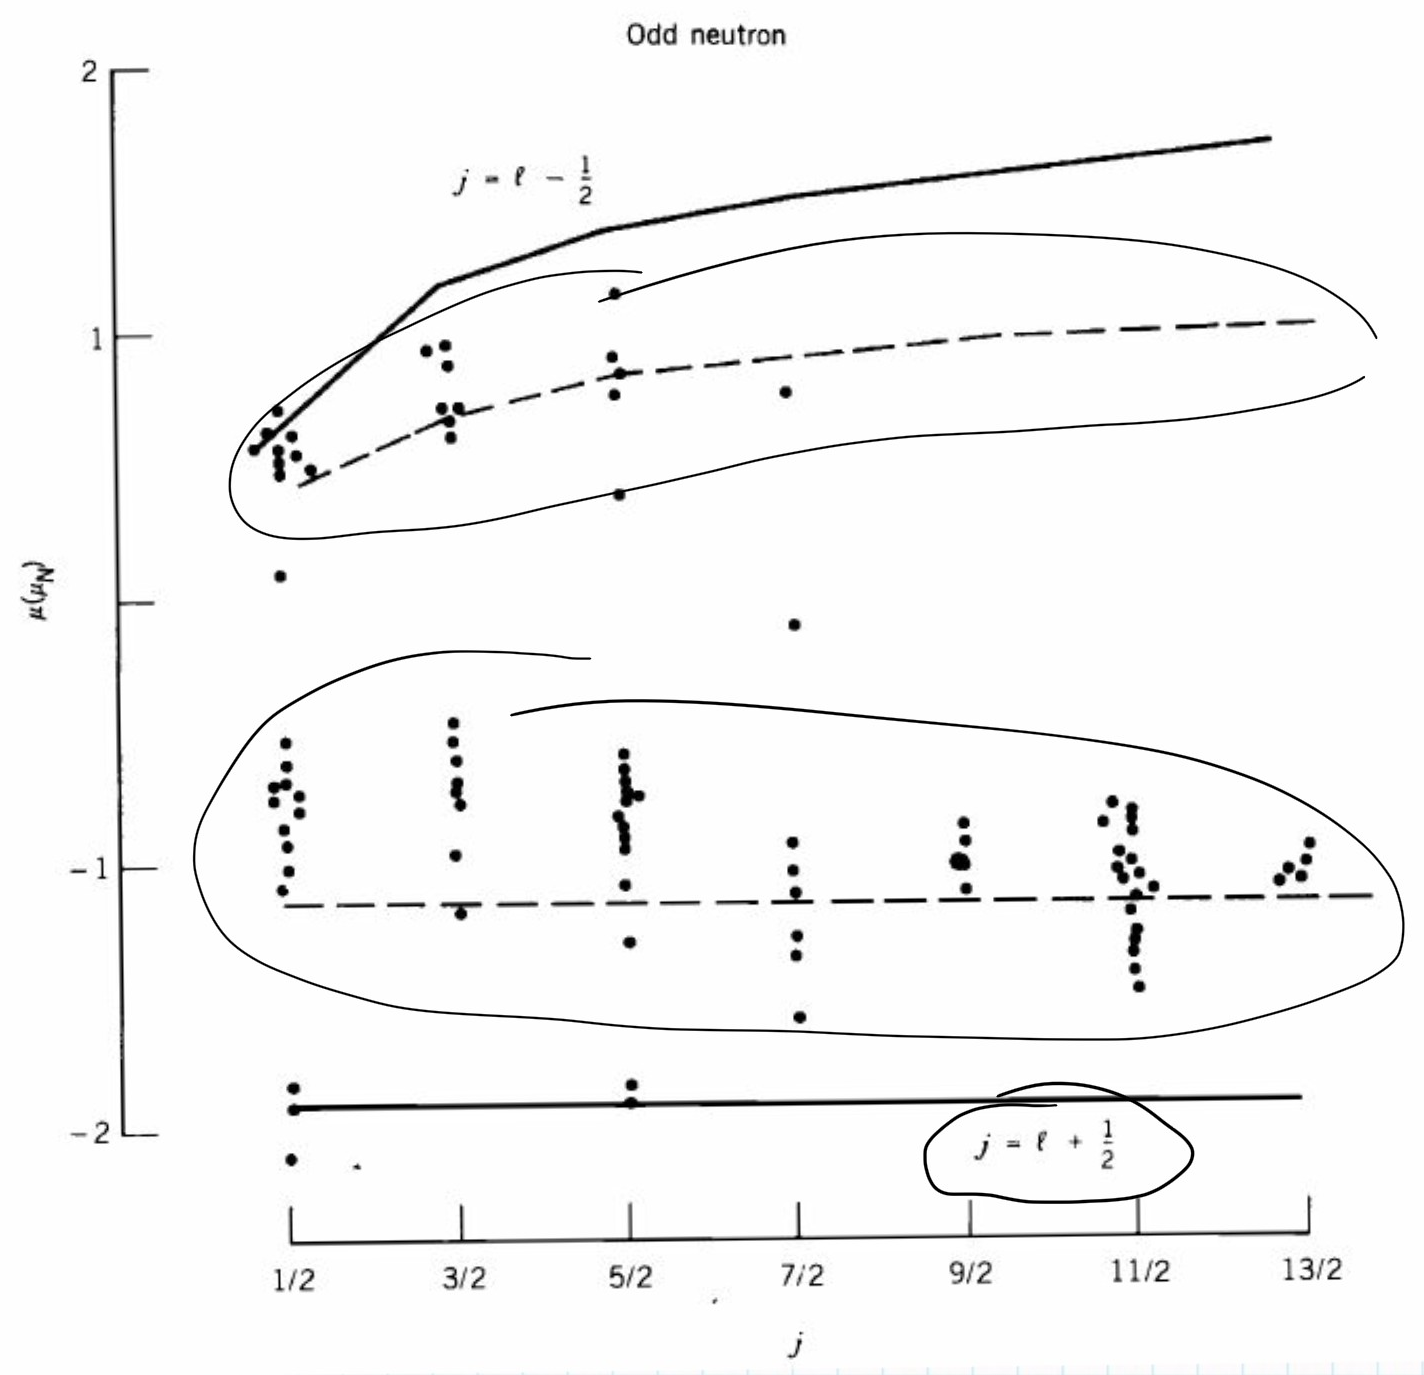
\includegraphics[scale=0.175]{Immagini/curve-Smith.png}
    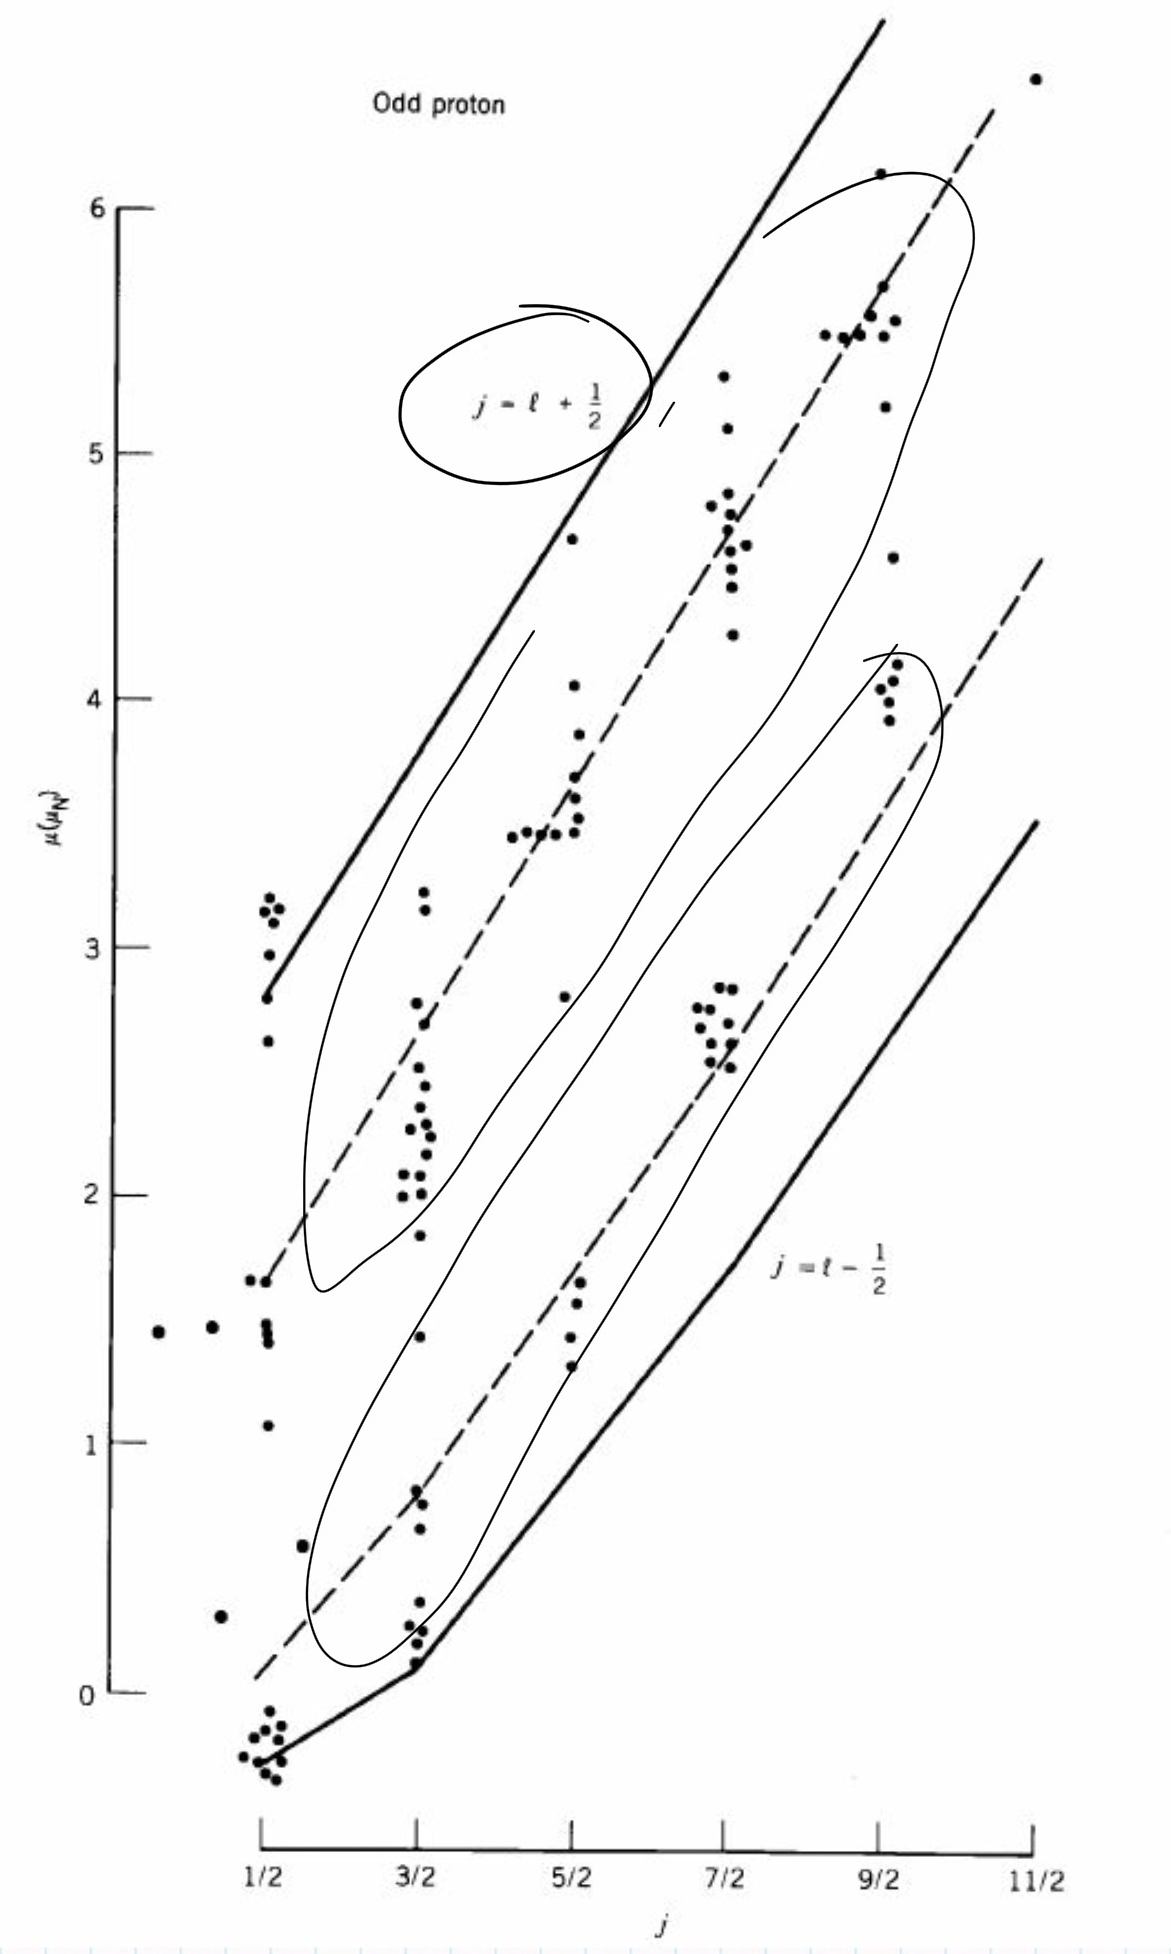
\includegraphics[scale=0.175]{Immagini/curve-Smith2.png}
    \caption{Andamenti dei momenti di dipolo magnetico per il neutrone a sinistra e per il protone a destra. La linea continua rappresenta le linee di Smith senza correzione, mentre quella tratteggiata tiene conto della \textit{medium modification}.}
    \label{curve}
\end{figure}

\begin{figure}[!h]
    \centering
    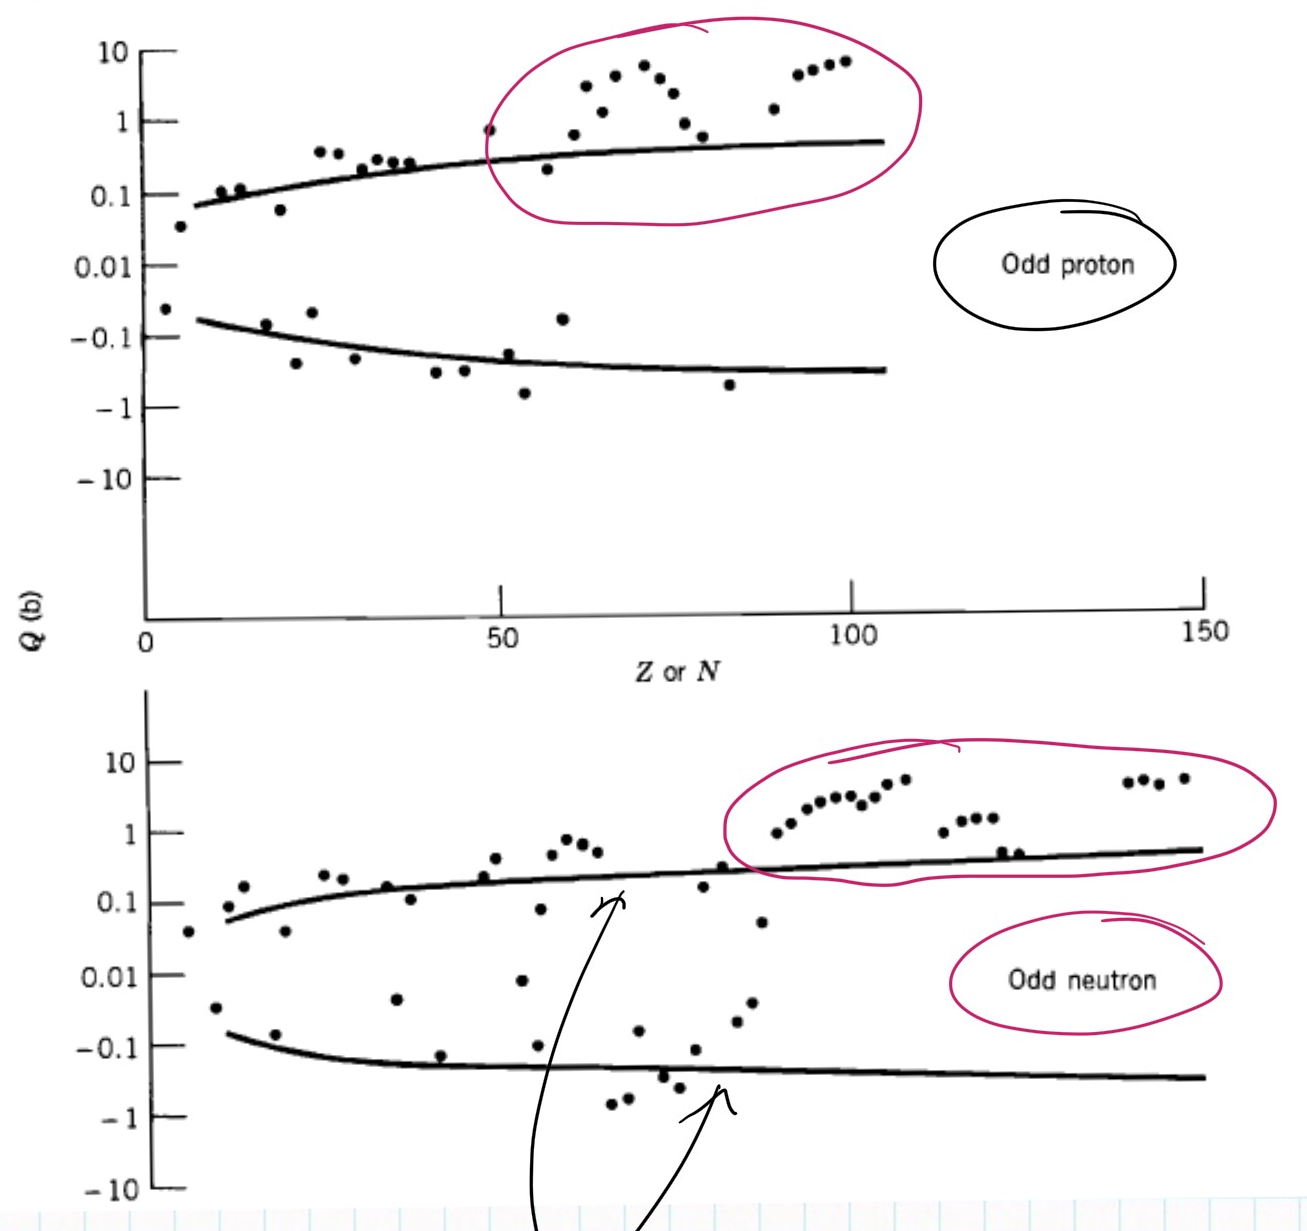
\includegraphics[scale=0.2]{Immagini/andamenti.png}
    \caption{Andamenti dei momenti di quadrupolo elettrico per il protone spaiato in alto e per il neutrone spaiato in basso.}
    \label{Q}
\end{figure}
\newpage